\section{Does Optimisation Close the Cost Gap?}\label{sec:opt}

A fair objection to \cref{sec:cost} is that no deployment verifies term by term: a real verifier batches
the work. We therefore optimised both verifiers and asked whether the gap closes.

\subsection{Optimisations}
\prov{Implementation}. Two optimisations are applied to both schemes.
\begin{enumerate}
\item \textbf{Multi-scalar multiplication (MSM).} The whole verification equation is evaluated in one
      native call (OpenSSL's \code{EC\_POINTs\_mul}) instead of one call per term. Sums whose coefficient
      is 1 (the repaired scheme's $\sum T_i$ and Verma's aggregate $R$) are plain point additions outside
      that call.
\item \textbf{A prepared roster.} An industrial fleet is fixed, so each sensor's point encodings and its
      certificate hash $h_0^i$ never change and are computed once per roster, not once per batch. For the
      repaired scheme the roster also caches $C_i=R_i+h_0^i\PTA$, because
      $u_iR_i+u_ih_0^i\PTA=u_iC_i$ folds two multi-scalar terms per signer into one. Verma's $h_0^i$
      already collapse into a single $\PTA$ term, so it has nothing equivalent to fold.
\end{enumerate}
In this best-effort shape the repaired scheme's multi-scalar call has $2n$ full-scalar terms
($u_iC_i$ and $v_ipk_i$) and Verma's has $n+1$ ($v_ipk_i$ and one $\PTA$ term): 1000 against 501 at
$n=500$. A test fixes this shape, so no coefficient-1 term can enter the call. Every optimised path is
checked against the reference implementation on both backends, for valid signatures and for each kind of
tampering.

\subsection{Results}
\prov{Experiment}. \Cref{fig:opt} shows the per-signer cost on P-256 at each stage. As specified, the
repaired scheme costs $169.5$~$\mu$s per signer against Verma's $71.5$ (ratio $2.37$). Fully optimised it
costs $53.7$ against $22.4$ (ratio $2.40$). Both schemes become about three times faster, and the ratio
does not move. Over four runs the ratio was $2.32$--$2.38$ as specified and $2.36$--$2.45$ optimised.

\begin{figure}[ht]
\centering
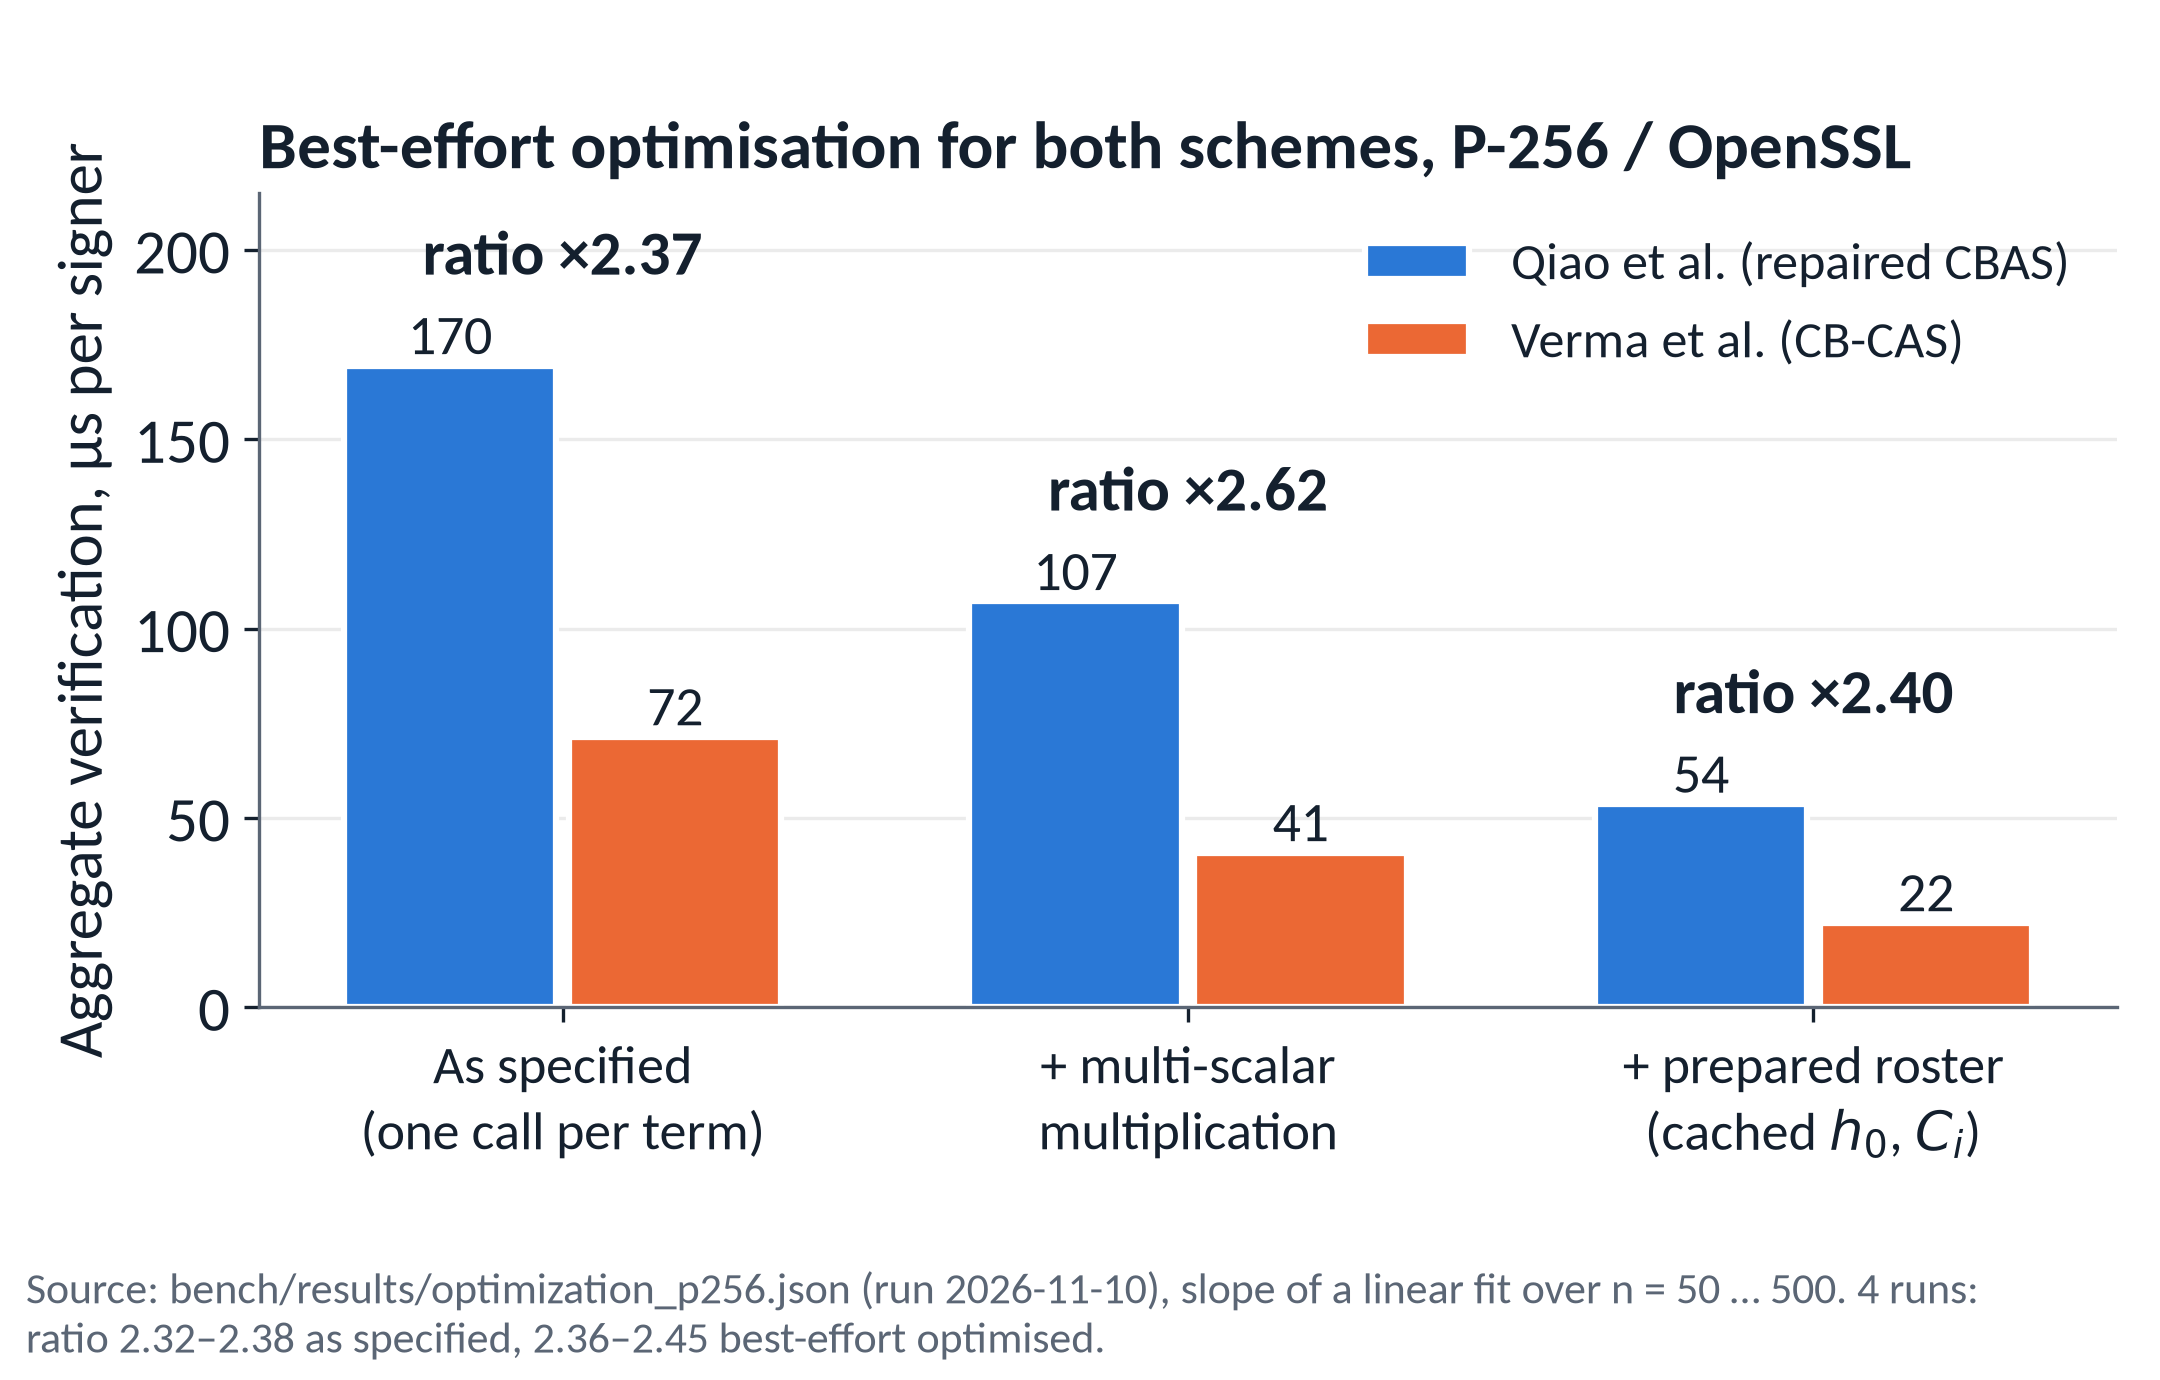
\includegraphics[width=0.85\linewidth]{figures/final_optimisation.png}
\caption{Per-signer aggregate-verification cost on P-256 at each optimisation stage, both schemes in
their best-effort shape. The middle stage is higher for the repaired scheme because it still recomputes
$h_0^i$ and its encodings for every batch.}
\label{fig:opt}
\end{figure}

On Ristretto255 libsodium offers no native multi-scalar routine, so only the roster helps. The ratio
barely moves: $2.02$--$2.20$ as specified and $1.99$--$2.14$ optimised. Which optimisation pays depends on the library rather than the scheme: OpenSSL keeps
points in projective coordinates, so additions are cheap and encoding costs an inversion, while libsodium
keeps a point as its encoding, so encoding is nearly free and additions are expensive.

The ratio stays a little above 2 because the repaired scheme needs two full-scalar terms per signer
against Verma's one, plus one more hash per signer and the $n$ additions for the $T_i$. Either way, the
paper's ratio of $1.00$ is not rescued by a good implementation.

\subsection{Two measurement mistakes, and what they teach}
Equal treatment means giving each scheme its own best-effort implementation, and we got it wrong twice,
once in each direction. Our first version gave the prepared roster to the repaired scheme only and
reported a ratio of $1.63$, which suggested that optimisation closes the gap. Our second version fed the
coefficient-1 $T_i$ into the multi-scalar call as $3n+1$ terms and did not cache $C_i$; it reported about
$3.0$ (between $2.95$ and $3.07$), which suggested the gap \emph{widens}. A review of our own presentation
caught the second error. With both schemes in their best-effort shape the ratio is about $2.4$, the same
as before optimisation. Comparing a careful implementation of one scheme with a careless one of the other
measures the implementations, not the schemes.

\paragraph{Signer side.} On the sensors, which are the constrained devices, caching the static encodings
speeds up \textsf{Sign} on P-256 from $74.8$ to $43.9$~$\mu$s ($1.70\times$) and leaves Ristretto255
unchanged. Group operations stay at $1\Te+2\Th$, and the nonce is still drawn fresh for every signature;
a test checks this, because a cached nonce would leak the keys (\cref{sec:nonce}).
